% Comentários Douglas
%  - Rever os objetivos específicos e geral para deixar mais explicativo e fechar melhor o escopo
%  - Materiais antes de métodos
%  - Trabalhos relacionados pode ser melhor explorados
%  - Fraco refereciamento em vários itens do texto
%  - Muitas palavras em inglês
%  - Melhorar requisito funcionais
%  - Falta um texto de suporte do visão geral
%  - Faltam diagramas para suportar a implementação (e não dos testes) junto ou talvez substituir trechos de código

% Comentários Tiago
%  - Destacar melhor características de tempo real: se não injetar nenhuma falta o seu sistema pode falhar?
%  - Destacar que o sistema é de tempo real e qual é o requisito de tempo real
%  - heartbit talvez seja a técnica para atrelar em teste de atender o requisito de tempo real.
%  - Plano de teste alinhados com os requisitos
%  - Diagramas de sequência (ou fluxograma) entre outros para descrever os testes 
%  - Analisar cronograma para realizar os testes

\chapter{Projeto}
\label{cap:proj}

\section{Visão Geral e Premissas}

\subsection{Visão Geral}

\subsection{Premissas}

% TODO: Termos em ingles
Será partido do ponto que ao menos o processador que executa o escalonador terá registradores de controle (Stack Pointer, Program Counter, Return Address) que sejam capazes de mascarar falhas. Apesar de ser possível executar os algoritmos reforçados com análise de fluxo do programa e adicionar redundância aos registradores, isso adiciona um grau a mais de complexidade que foge do escopo do trabalho, e, como mencionado na \autoref{sec:trabRel}, a memória fora do banco de registradores pode ser 2 ordens de magnitude mais sensível à eventos disruptivos @ReliabilityArmCortexUnderHeavyIons.

Portanto, todos os testes subsequentes assumirão ao menos uma quantia mínima de tolerância do núcleo monitor, tendo foco na detecção de falhas de memória, passagem de mensagens e resultados dos co-processadores.

Com o fim de reduzir o tamanho do executável e manter o fluxo de execução mais previsível não será utilizado mecanismo de exceção com stack unwinding ou RTTI (Runtime Type Information), ao invés, erros de validação devem ser cuidados explicitamente com valores ou através de callbacks.

Necessariamente, é preciso também presumir que testes sintéticos possam ao menos aproximar a performance do mundo real, ou ao menos prever o pior caso possível com grau razoável de acurácia. O uso de testes sintéticos não deve ser um substituto para a medição em uma aplicação real, porém, uma bateria de testes com injeção artificial de falhas pode ser utilizada para verificar as tendências e overheads relativos introduzidos, mesmo que não necessariamente reflitam as medidas absolutas do produto final.

Portanto, será assumido que os resultados extraídos de injeção de falhas artificiais, apesar de menos condizentes com os valores absolutos de uma aplicação e não sendo substitutos adequados na fase de aprovação de um produto real, são ao menos capazes para realizar uma análise quanto ao overhead proporcional introduzido, e devido à sua facilidade de realização e profundidade de inspeção possível, serão priorizados inicialmente neste projeto.

\section{Metodologia}

\subsection{Materiais}

% TODO: sumarizar, mais diagramas, melhorar coesao deixar um pouco mais segmentado e com conexoes entre os topicos, aqui e em metodos. referenciar as figuras

Será utilizada a linguagem C++ com o compilador GCC (ou Clang), o alvo principal do trabalho será um microcontrolador STM32F103C8T6 "Bluepill" 32-bits da arquitetura ARMv7-M, como visto na \autoref{fig:stm32Bluepill}.

\begin{figure}[H]
    \centering
    \caption{Diagrama da STM32F103C8T6 ("Bluepill")}
    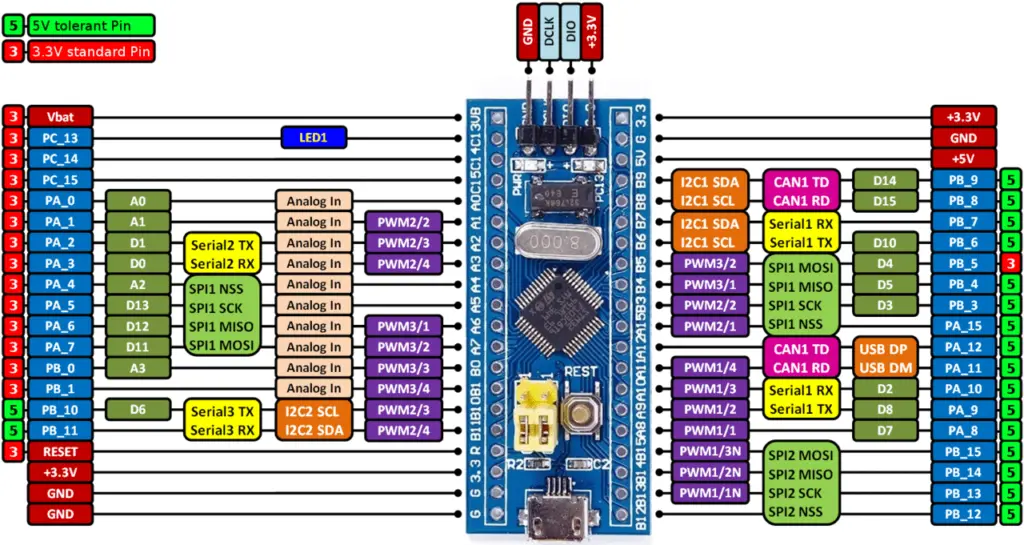
\includegraphics[width=0.80\textwidth]{assets/stm32_bluepill.png}
    \caption*{Fonte: \cite{STMBoardProductPage}}
    \label{fig:stm32Bluepill}
\end{figure}

Para a injeção de falhas será utilizado o depurador GDB em conjunto com uma ferramenta de depuração de hardware ST-LINK (\autoref{fig:stLink}), a comunicação do ST-LINK é feita via USB com o computador e via JTAG com o microcontrolador alvo, também será usado em conjunto uma IDE fornecida pelo mesmo fabricante, a STM32Cube IDE.

\begin{figure}[H]
    \centering
    \caption{ST-LINK/V2}
    
\includegraphics[width=0.50\textwidth]{assets/st_link.png}
    \caption*{Fonte: \cite{STLinkProductPage}}
    \label{fig:stLink}
\end{figure}

\begin{figure}[H]
    \centering
    \caption{ST-LINK/V2}
    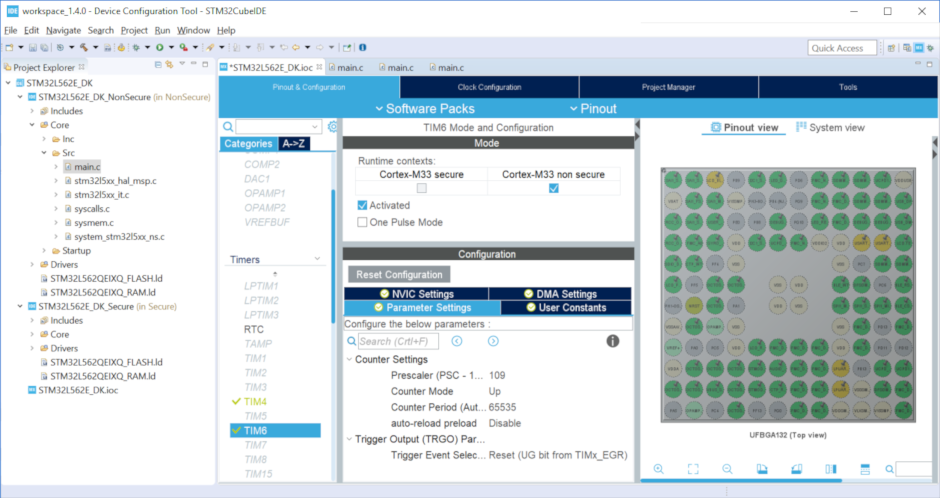
\includegraphics[width=0.80\textwidth]{assets/stmcube_ide.png}
    \caption*{Fonte: \cite{STMCubeProductPage}}
    \label{fig:stLink}
\end{figure}

% #sourced_image(
%   caption: [STMCube IDE],
%   source: "STMCubeProductPage",
%   image("assets/stmcube_ide.png"))

Durante a fase de desenvolvimento dos algoritmos será utilizado o QEMU juntamente com as ferramentas anteriormente citadas, assim como sanitizadores de memória e condições de corrida (ASan, TSan, UBSan) para auxiliar na detecção de erros mais cedo durante o desenvolvimento.

O sistema operacional de tempo real escolhido foi o FreeRTOS, por ser extensivamente testado e documentado e prover um escalonador totalmente preemptivo com um custo espacial relativamente pequeno, além disso, os contribuidores do FreeRTOS mantém uma lista grande de versões para diferentes arquiteturas e controladores, facilitando drasticamente o trabalho ao não ter que criar uma HAL do zero.

\subsection{Métodos}

% TODO: sumarizar, mais diagramas, melhorar coesao
Serão utilizadas técnicas de detecção e tolerância à falhas implementadas em software, duas das técnicas são diretamente associadas à interface de tarefa, uma serve como tarefa supervisora e as outras duas servem como suporte. Os detalhas específicos de cada técnica serão abordados posteriormente.

% TODO: sumarizar, mais diagramas, melhorar coesao
Para executar a injeção lógica em software será utilizado um ambiente virtual (QEMU) emulando a mesma arquitetura de processador juntamente com o depurador GDB e funções de injeção implementadas diretamente nos programas utilizando callbacks para disparar uma falha, a emissão de falhas ocorrerá periodicamente de forma parametrizada. A injeção lógica em software não é o objetivo final do trabalho mas serve como uma validação prévia durante o processo de desenvolvimento assim como uma possível contingência.

% TODO: sumarizar, mais diagramas, melhorar coesao
A injeção lógica em hardware é realizada com ferramentas do próprio fabricante do microcontrolador (detalhas na seção seguinte), o fluxo geral da injeção consiste em carregar o binário executável (no formato ELF) no micro controlador utilizando o ST-LINK, após isso, o programa será iniciado e será feita uma injeção de falhas via sessão do depurador GDB associado ao link.

% TODO: sumarizar, mais diagramas, melhorar coesao
A coleta de métricas é realizada com os mecanismos de monitoramento do sistema FreeRTOS juntamente com contadores de incremento atômico, o tempo de execução das tarefas, seu espaço de memória utilizado e o número de falhas detectadas (e causadas) será armazenado em uma estrutura que residirá em um segmento de memória que é deliberadamente isento de falhas, servindo similarmente à uma "caixa preta" do sistema.

% TODO: sumarizar, mais diagramas, melhorar coesao
Para simular uma carga de trabalho mais condizente com a aplicações reais, serão utilizados 2 programas de exemplo, um processador de sinal digital assíncrono e um programa que realiza uma convolução bidimensional, estes programas são executados e expostos à falhas que espera-se que os mecanismos de tolerância sejam capazes de detectar. Detalhamento destes programas pode ser encontrado no capítulo do *Plano de Verificação*.

% TODO: sumarizar, mais diagramas, melhorar coesao
Visando a reutilização de código e abstração, será utilizada uma interface que generaliza um objeto de tarefa, como um objeto que realiza despache dinâmico necessita de uma tabela de despache virtual (V-Table), é necessário tomar cuidado adicional pois a própria tabela pode ser sujeita à falhas. Será aplicado uma replicação simples dos ponteiros de função da vtable, com o custo adicional de 2 comparações por chamada de método. Espera-se que este custo não será significativo pois os métodos da interface não são chamados com uma frequência alta.


\section{Análise de requisitos}
\label{sec:req}

\begin{quadro}[H]
    \centering
    \caption{Requisitos funcionais}
    \begin{tabular}{|p{0.125\textwidth}|p{0.8\textwidth}|}
        \hline
        \rowcolor[HTML]{C0C0C0}
        \textbf{Requisito} & \textbf{Descrição}  \\
        \hline
        
        \textbf{RF01} & aaaaaaaaa \\ 
        \hline

        \textbf{RF02} & bbbbbbbbb \\
        \hline
        
        \textbf{RF03} & ccccccccc \\
        \hline
        
        \textbf{RF04} & ddddddddd \\
        \hline
        
        \textbf{RF05} & eeeeeeee \\
        \hline
    \end{tabular}
    \label{tab:rf}
\end{quadro}

\begin{quadro}[H]
    \centering
    \caption{Requisitos não funcionais}
    \begin{tabular}{|p{0.125\textwidth}|p{0.8\textwidth}|}
        \hline
        \rowcolor[HTML]{C0C0C0}
        \textbf{Requisito} & \textbf{Descrição}  \\
        \hline
        
        \textbf{RNF01} & aaaaaaaaa \\ 
        \hline

        \textbf{RNF02} & bbbbbbbbb \\
        \hline
        
        \textbf{RNF03} & ccccccccc \\
        \hline
        
        \textbf{RNF04} & ddddddddd \\
        \hline
        
        \textbf{RNF05} & eeeeeeee \\
        \hline
    \end{tabular}
    \label{tab:rf}
\end{quadro}

\subsection{Interface}

Para melhor generalizar o uso das técnicas, utiliza-se de uma abstração da estrutura de tarefa para facilitar a utilização de diferentes técnicas de execução sem necessitar de alterações significativas por parte do usuário da interface.

% O "corpo" de um tarefa é simplesmente a função que executa após a tarefa ter sido inicializada. Será utilizado uma assinatura simples permitindo a passagem de um parâmetro opaco por referência. Este parâmetro pode ser o argumento primordial da tarefa ou um contexto de execução. Tarefas são expressas na forma de uma interface, que contém métodos que podem ser implementados de acordo com a necessidade da tarefa.

Uma mensagem envelopa um pacote de dados qualquer para que possa ser enviado de forma assíncrona por uma , o ordenamento dos tipos é importante, o pacote precisa ser o último membro para serialização de estruturas de tamanho arbitrário, a distribuição dos campos na memória é demonstrada na \autoref{fig:messageStruct}. 

\begin{figure}[H]
    \centering
    \caption{Layout de uma mensagem}
    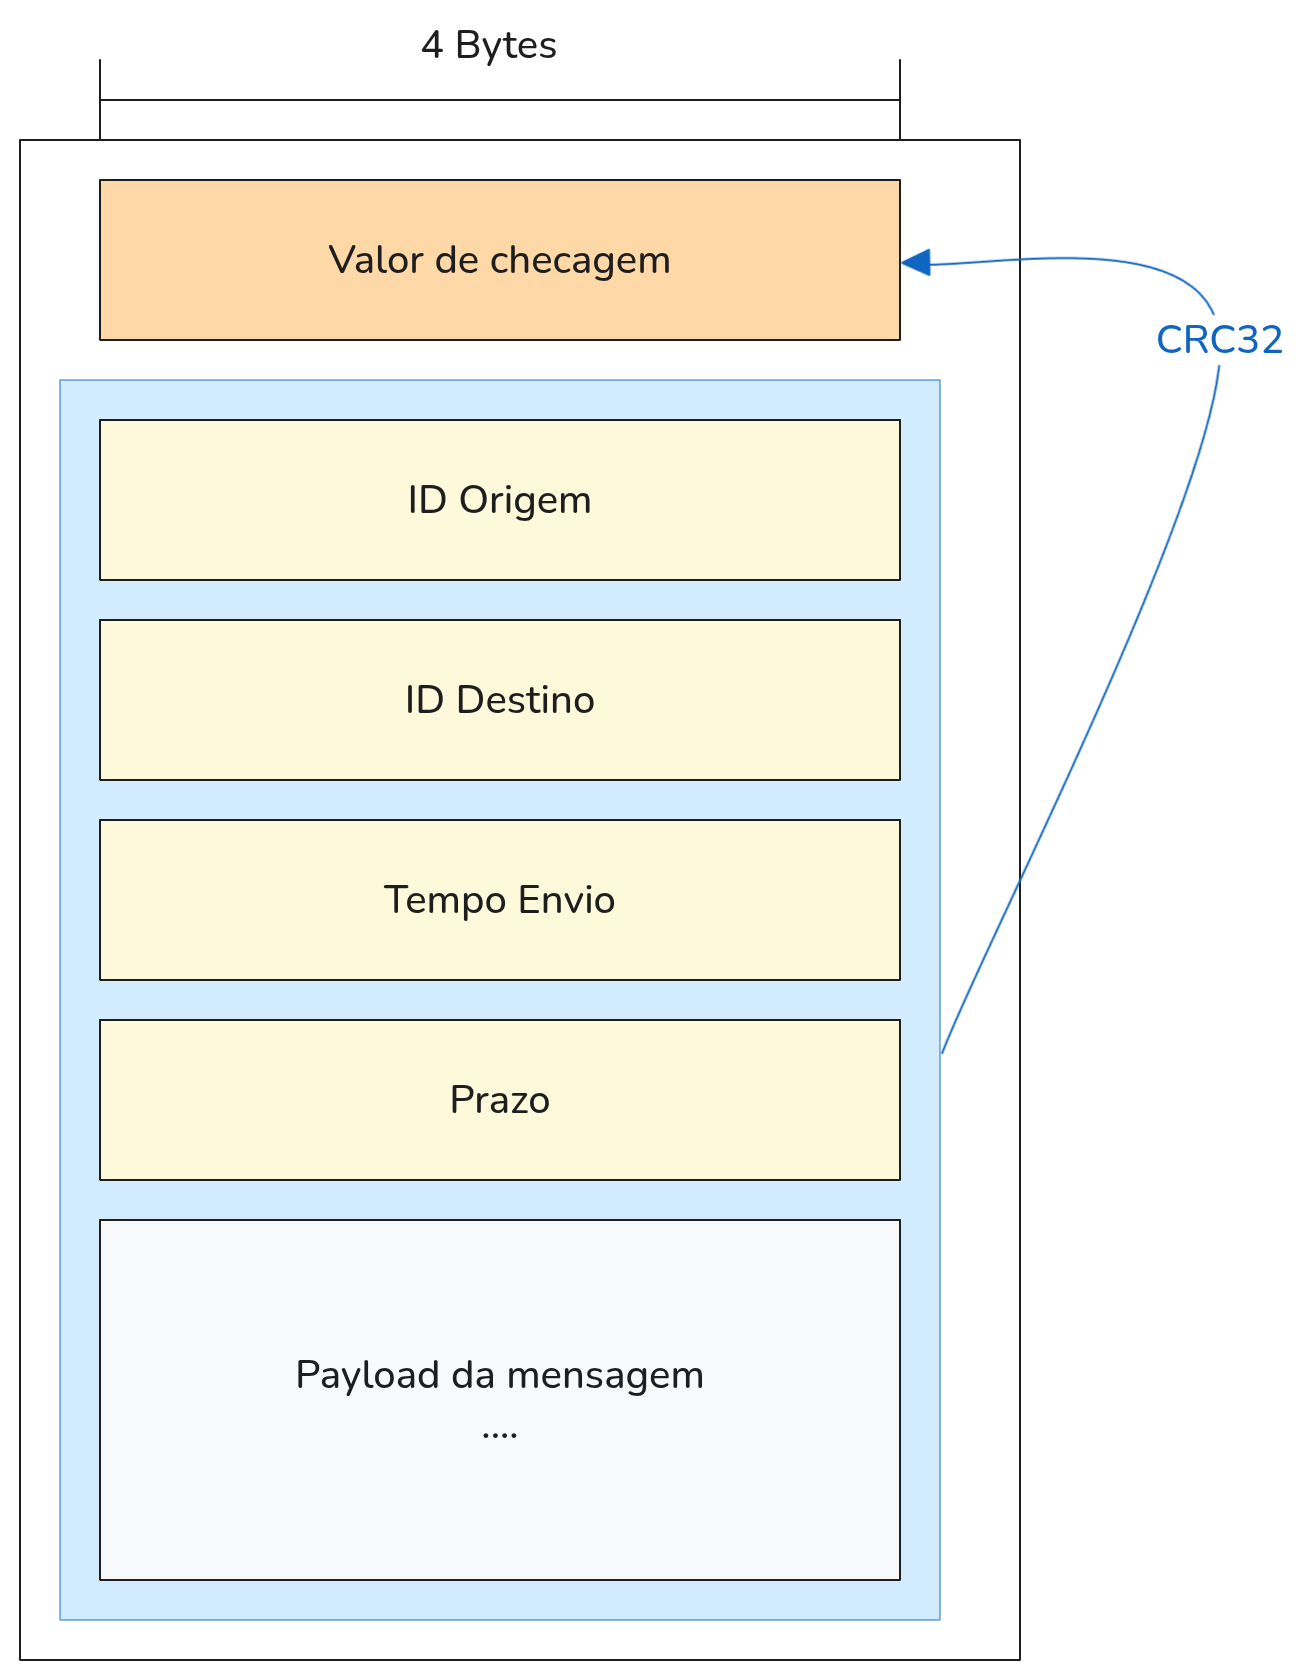
\includegraphics[width=0.60\textwidth]{assets/payload_layout.png}
    \caption*{Fonte: Elaborada pelo autor}
    \label{fig:messageStruct}
\end{figure}

\subsection{Algoritmos e Técnicas}

Para a implementação da funcionalidade de tolerância à falhas, algumas das técnicas previamente abordadas no \autoref{cap:fund} serão utilizadas. O detalhamento sobre a implementação será abordado nesta seção.

\subsubsection{CRC: Cyclic Redundancy Check}
% TODO fazer!

\subsubsection{Redundância Modular}

Para a aplicação da redundância modular, neste caso a redundância modular tripla, será feito a replicação concorrente da tarefa, cada tarefa possui um espaço de pilha próprio e são escalonadas de forma convencional pelo FreeRTOS. O corpo das tarefas não é replicado, e continua como parte de memória para apenas leitura e execução, um exemplo da relação de réplicas de tarefas executando em relação ao resto do sistema pode ser observado. 

\begin{figure}[H]
    \centering
    \caption{Diagrama de bloco de Redundância modular}
    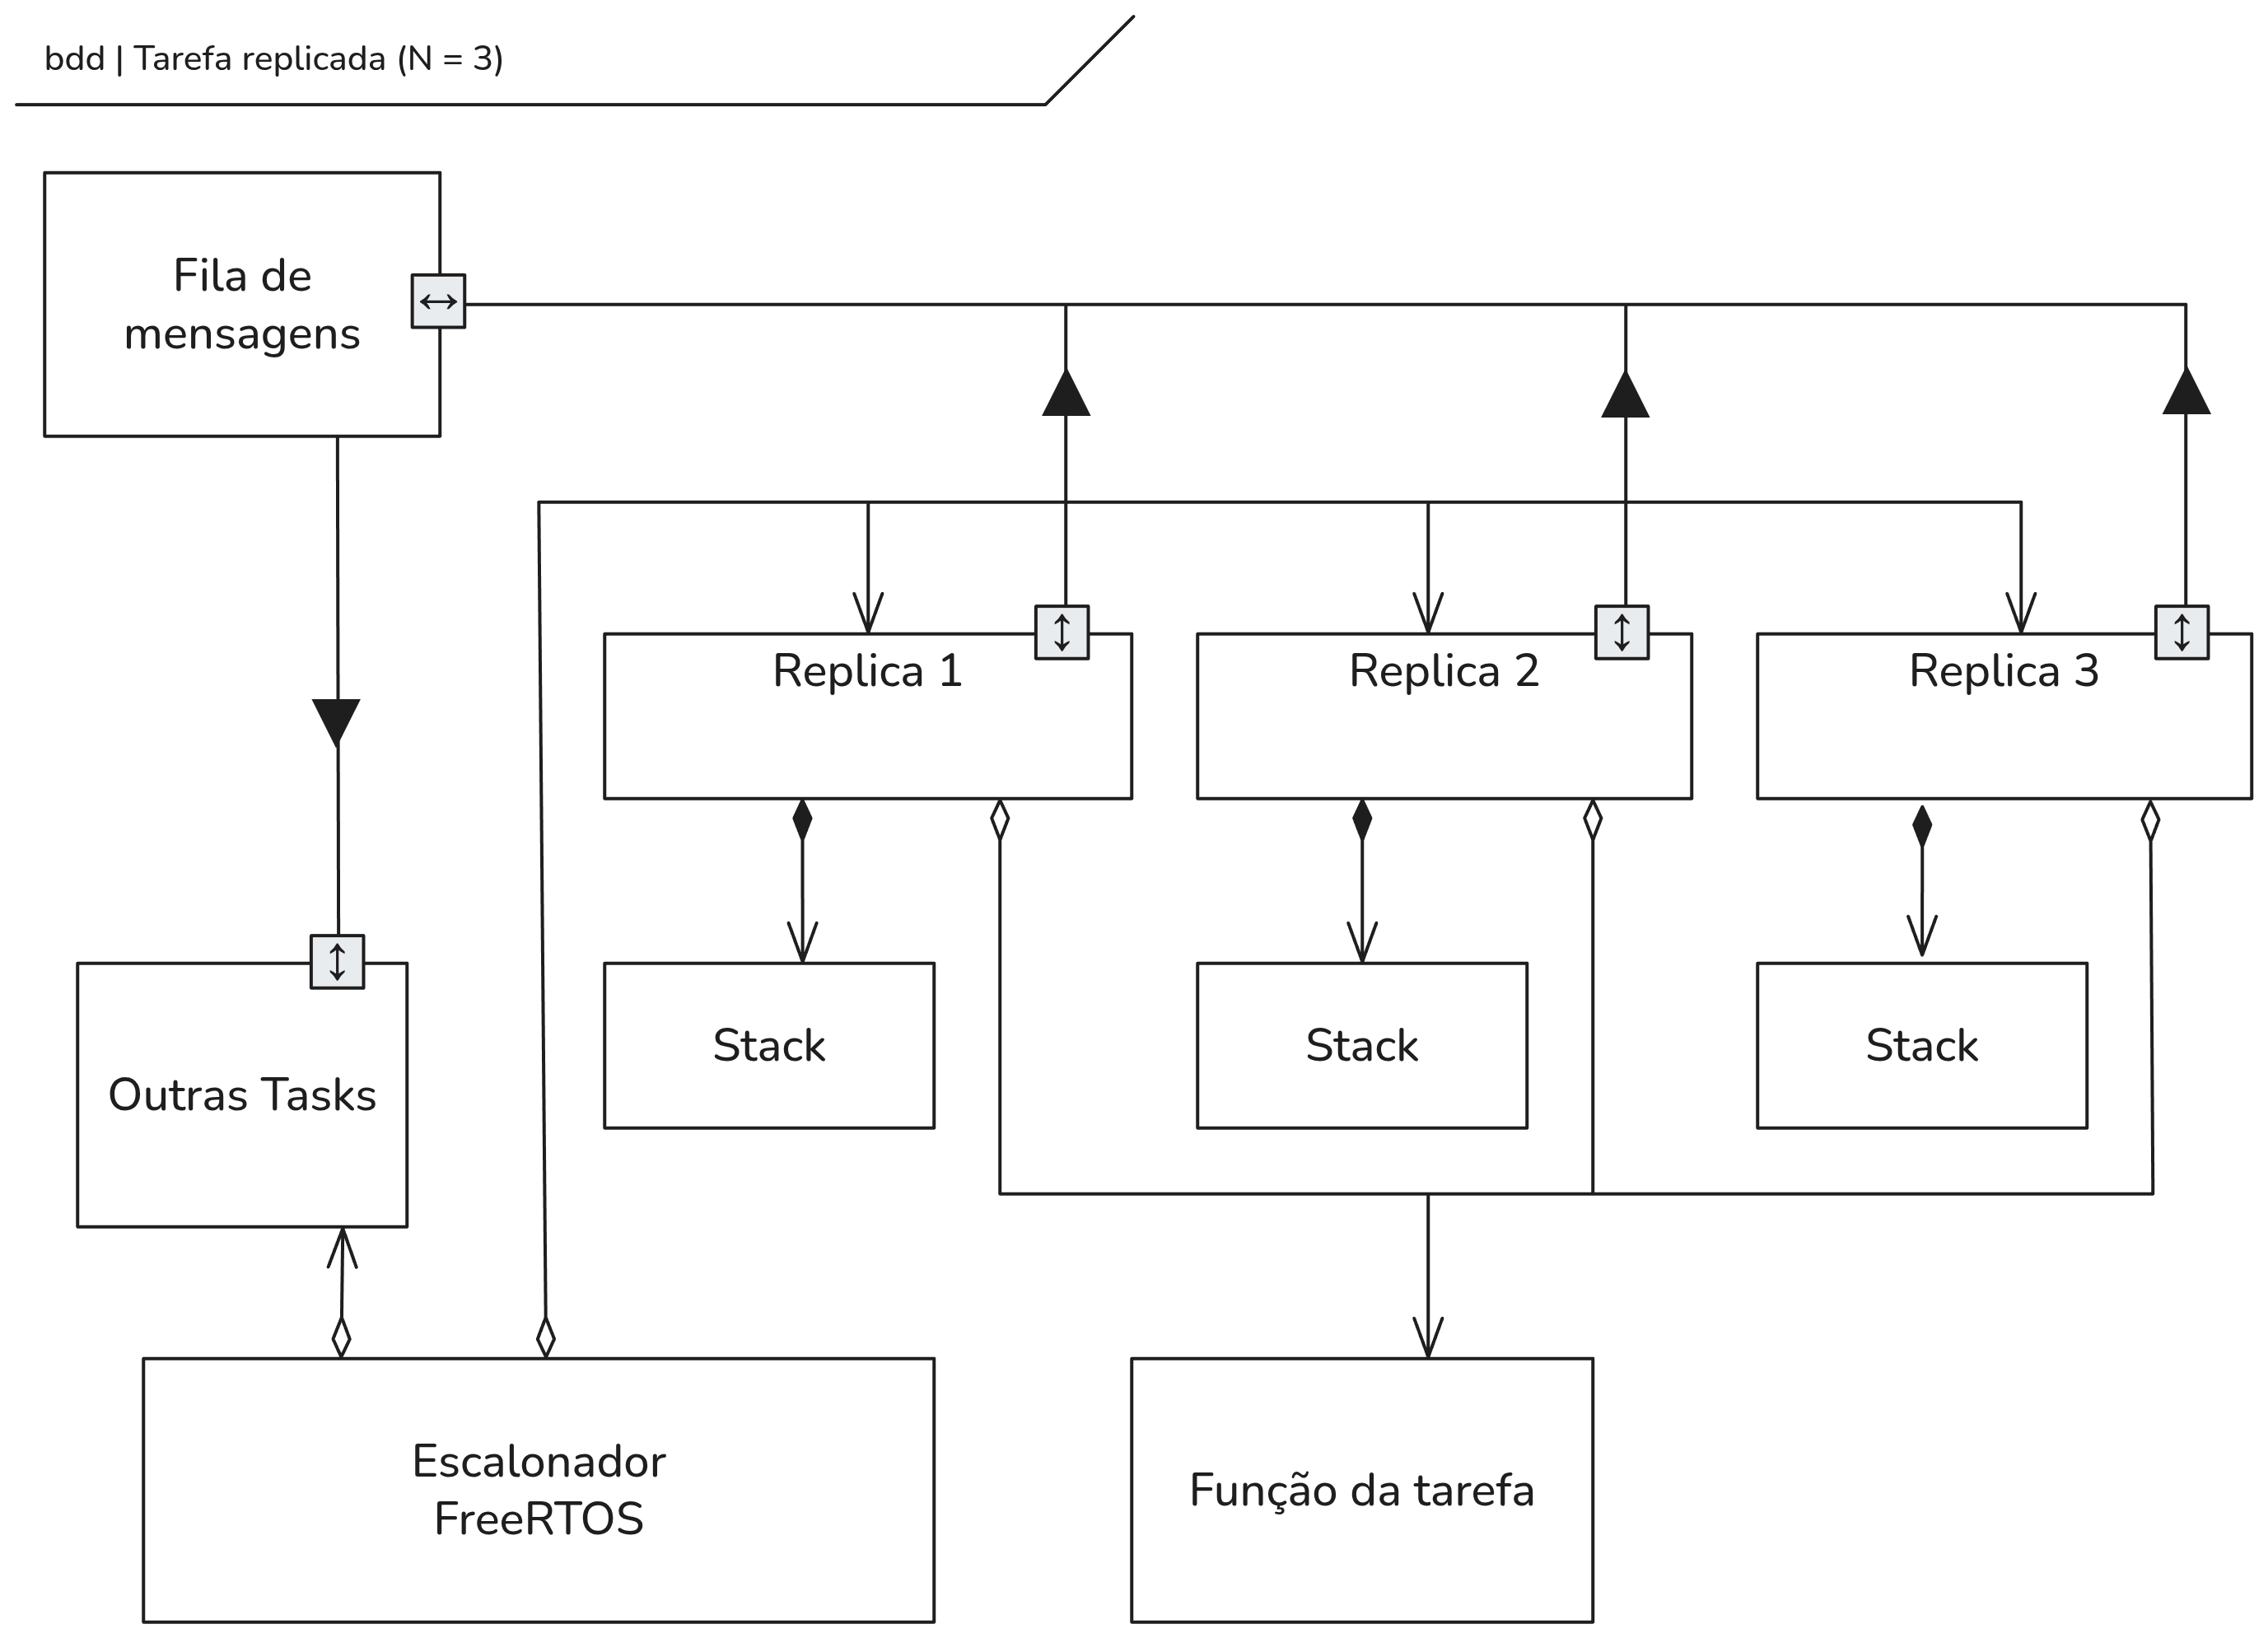
\includegraphics[width=0.975\textwidth]{assets/tmr_bdd.png}
    \caption*{Fonte: Elaborada pelo autor}
    \label{fig:messageStruct}
\end{figure}

\subsubsection{Reexecução}

% TODO disagrama

\section{Plano de Verificação}

% \begin{quadro}[H]
%     \centering
%     \noindent
%     \caption{Requisitos não funcionais}
%     \begin{tabular}{|p{0.15\textwidth}|p{0.8\textwidth}|}
%         \hline
%         \rowcolor[HTML]{C0C0C0}
%         \textbf{Requisito} & \textbf{Descrição}  \\
%         \hline
%         \textbf{RNF01} & O algoritmo de CNN deve ser treinado em Python com as bibliotecas TensorFlow, Keras e scikit-learn\\
%         \hline
%         \textbf{RNF02} & A CNN embarcada deverá ser desenvolvida usando as bibliotecas TensorFlow Lite e/ou TinyML\\
%         \hline
%         \textbf{RNF03} & O algoritmo de CNN deve ser implementado em linguagem C para ser embarcado\\
%         \hline
%         \textbf{RNF04} & O algoritmo de CNN deve ser embarcado no microcontrolador ESP32 e/ou Raspberry Pi Pico\\
%         \hline
%         \textbf{RNF05} & A memória consumida pelo algoritmo não deve ser maior que 4 MB\\
%         \hline
%         \textbf{RNF06} & A CNN embarcada deve ser implementada usando ESP-IDF para ESP32\\
%         \hline
%         \textbf{RNF07} & A CNN embarcada deve ser implementada usando Pico C/C++ SDK\\
%         \hline
%     \end{tabular}
%     \label{tab:rnf}
% \end{quadro}

